\chapter{Seguimiento del proyecto}

Este capítulo describe el transcurso real de cada una de las cinco iteraciones que componen el desarrollo del proyecto, detallando los avances técnicos alcanzados y la evolución visual del sistema a lo largo del tiempo. El desarrollo se organizó siguiendo una metodología iterativa e incremental, lo que permitió incorporar funcionalidad de forma progresiva, validar cada bloque antes de avanzar al siguiente y responder a los cambios de diseño que surgieron durante el proceso. Cada iteración partía de los entregables de la anterior y tenía definidos unos objetivos concretos cuyo cumplimiento se verificó al finalizar cada fase.

% ─────────────────────────────────────────────────────────────────────────────
\section{Iteración 1: Núcleo jugable y lógica básica}
% ─────────────────────────────────────────────────────────────────────────────

Esta primera fase se centró en la implementación de la base jugable, tenía como objetivo principal crear un \textit{Producto Mínimo Viable} funcional. En esta etapa, el videojuego carecía por completo de elementos estéticos, menús o \textit{feedback} visual y sonoro, centrándose exclusivamente en la validez de los movimientos y la resolución de combates.

Durante esta iteración se utilizaron \textit{placeholders} (elementos provisionales) para representar todas las entidades del videojuegos. La interfaz de despliegue consistía únicamente en botones con texto plano como se puede ver en la Figura \ref{fig:it1_interfaz}, y las piezas se diferenciaban solo por colores e iconos esquemáticos sobre formas cuadradas. Como detalle de la imagen, también se pueden apreciar que los nombres de las piezas no reflejaban las definitivas del producto final, ya que se fueron haciendo cambios según se volvía a dar una vuelta a sus conceptos durante el desarrollo, o se implementaban su apariencia.

\begin{itemize}
	\item \textbf{Piezas con rango:} Identificadas por un número según su valor de combate.
	\item \textbf{Núcleo de energía:} Representado por un signo de exclamación (!).
	\item \textbf{Torretas:} Identificadas mediante una letra "T".
\end{itemize}

La elección del color de las piezas responde a criterios de usabilidad y psicología del color básicos que se aplicaron casi de manera inconsciente, utilizando el azul para el jugador por su asociación con la calma y la seguridad, mientras que el naranja para el rival facilita un contraste visual inmediato y resalta la naturaleza competitiva y de alerta frente a las unidades enemigas.

\begin{figure}[H]
	\centering
	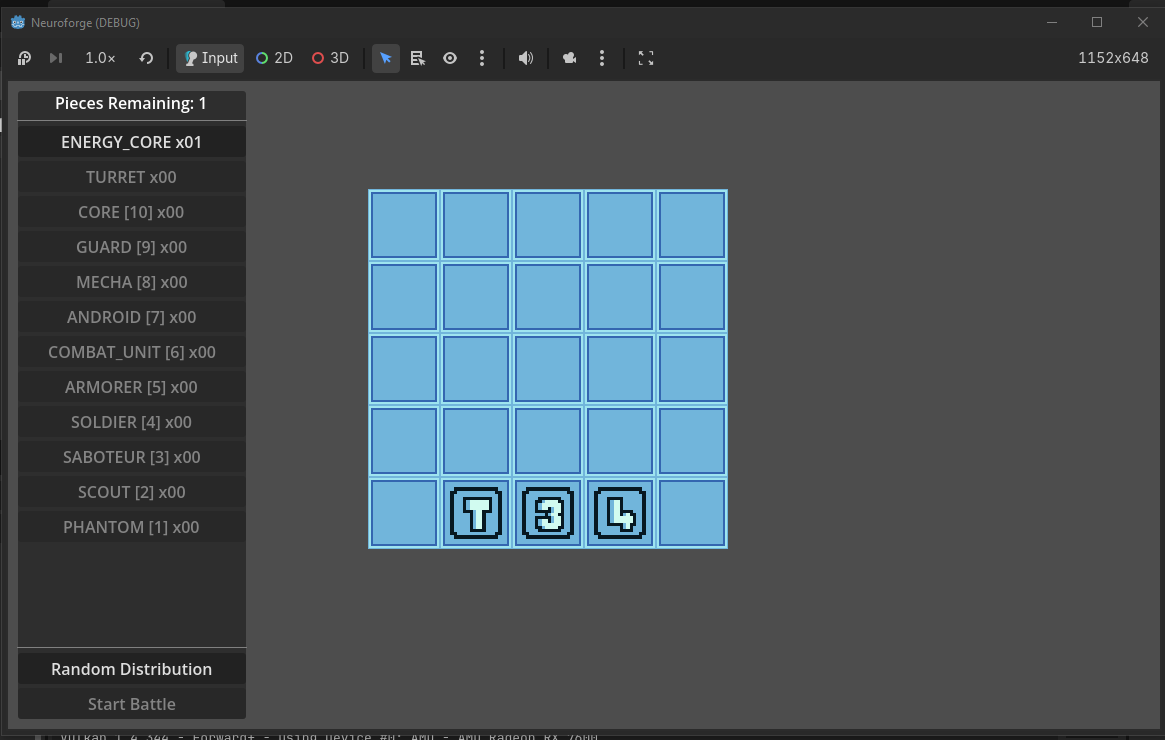
\includegraphics[width=\textwidth]{../Imagenes/it1_despliegue_cerca}
	\caption{Detalle de la interfaz de despliegue inicial basada en botones de texto.}
	\label{fig:it1_interfaz}
\end{figure}

El tablero utilizaba una codificación de colores básica para la retroalimentación visual del usuario:
\begin{itemize}
	\item \textbf{Gris:} Casillas intransitables que actúan como obstáculos permanentes.
	\item \textbf{Azul:} Casillas de agua o vacío. En esta fase no existía distinción visual entre las zonas de despliegue del jugador y de la inteligencia artificial, lo que dificultaba el posicionamiento inicial para alguien que no conociera el diseño del videojuego.
	\item \textbf{Verde:} Resaltado de casillas disponibles para movimiento tras seleccionar una pieza propia.
	\item \textbf{Rojo:} Indicador de casilla de combate inminente al seleccionar un objetivo enemigo.
\end{itemize}

La interacción era puramente lógica y carecía de retroalimentación visual. Los movimientos y combates eran instantáneos, sin animaciones de transición. Esta inmediatez provocaba problemas de seguimiento de la partida, ya que en ocasiones resultaba difícil saber que jugada realizado por el bot después del movimiento del jugador. 

Asimismo, no existía un flujo de partida completo, al finalizar el encuentro por la captura del núcleo, el sistema no mostraba pantallas de victoria o derrota, limitándose a imprimir un mensaje en la terminal de depuración de Godot y a detener la ejecución del videojuego como se puede observar en la Figura \ref{fig:it1_juego2}. Tampoco se implementaron menús de pausa, opciones ni efectos de sonido. En la Figura \ref{fig:it1_juego1} se pueden observar distintas partidas y situaciones del productor de la primera iteración. La iteración acabo dentro del plazo establecido.

\begin{figure}[H]
	\centering
	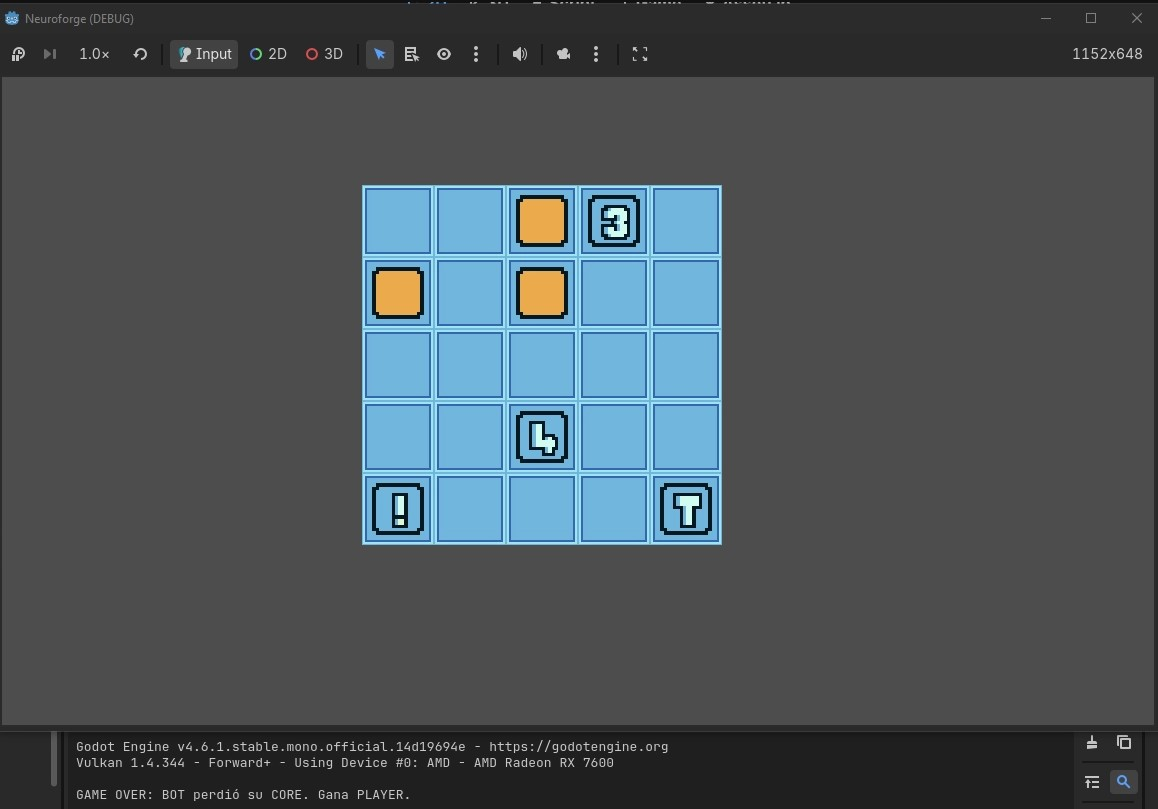
\includegraphics[width=\textwidth]{../Imagenes/it1_juego2}
	\caption{Mensaje de final de partida en la Iteración 1}
	\label{fig:it1_juego2}
\end{figure}

\begin{figure}[H]
	\centering
	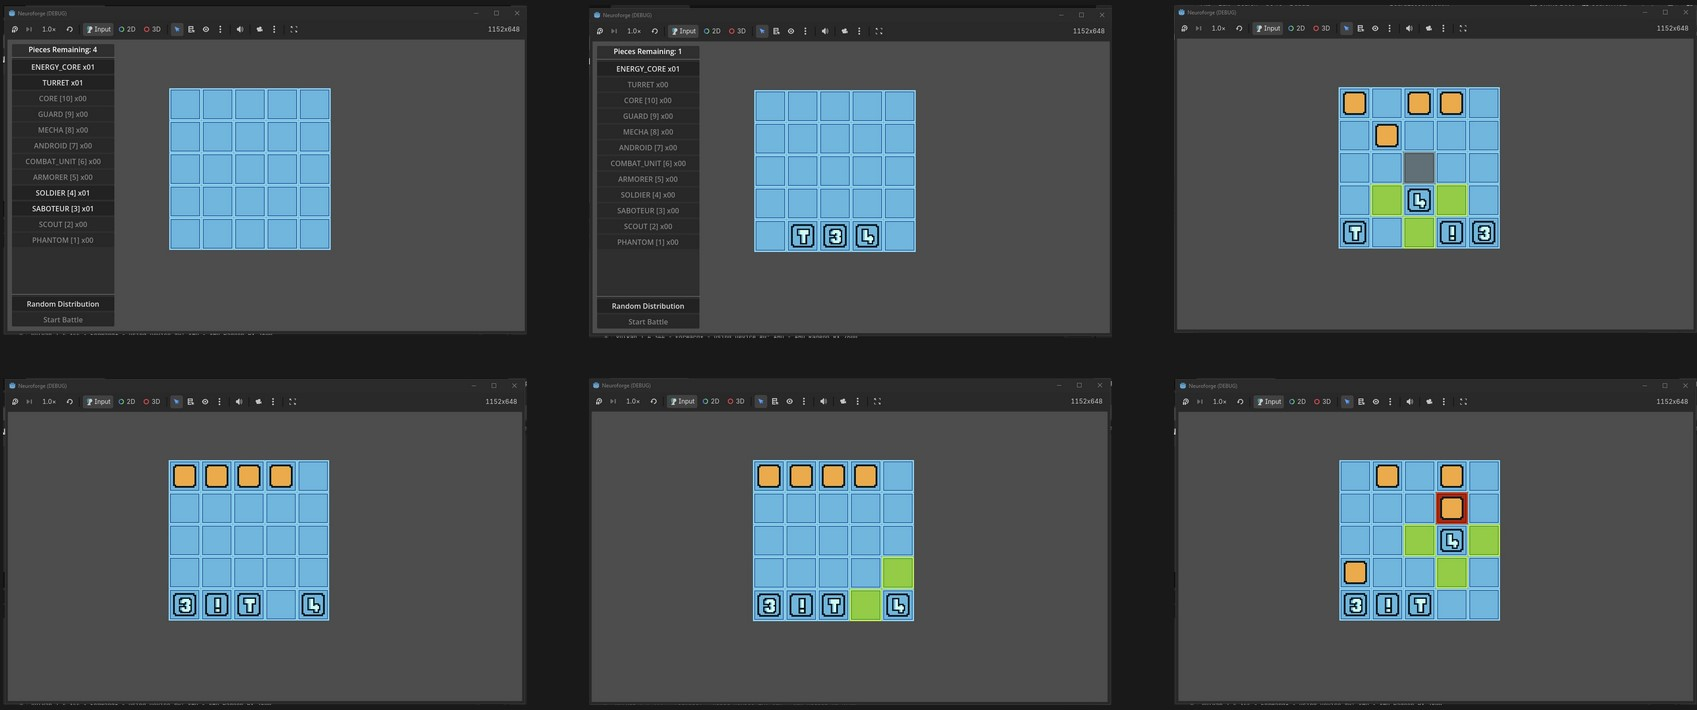
\includegraphics[width=\textwidth]{../Imagenes/it1_juego1}
	\caption{Capturas del juego durante la Iteración 1.}
	\label{fig:it1_juego1}
\end{figure}

% ─────────────────────────────────────────────────────────────────────────────
\section{Iteración 2: Interfaz de usuario y pulido visual}
% ─────────────────────────────────────────────────────────────────────────────
En esta segunda fase, el desarrollo se centró en transformar los elementos provisionales de la iteración anterior en una interfaz de usuario (UI) coherente, intuitiva y visualmente atractiva. Para la planificación y el diseño de estas interfaces se utilizó la herramienta \textit{draw.io}, permitiendo bocetar la disposición de los elementos antes de su implementación definitiva en el motor.

\subsubsection{Interfaz de partida}

La interfaz principal de videojuego se diseñó con el objetivo de centralizar toda la información necesaria para el jugador sin sobrecargar la vista. En su primera concepción, el boceto mostraba un tablero central rodeado por los indicadores de piezas restantes a ambos lados y un historial de movimientos situado en la esquina inferior izquierda. El estado del turno se indicaba mediante un texto descriptivo en la parte superior como se puede observar en la Figura \ref{fig:boceto_partida_v1}.

\begin{figure}[H]
	\centering
	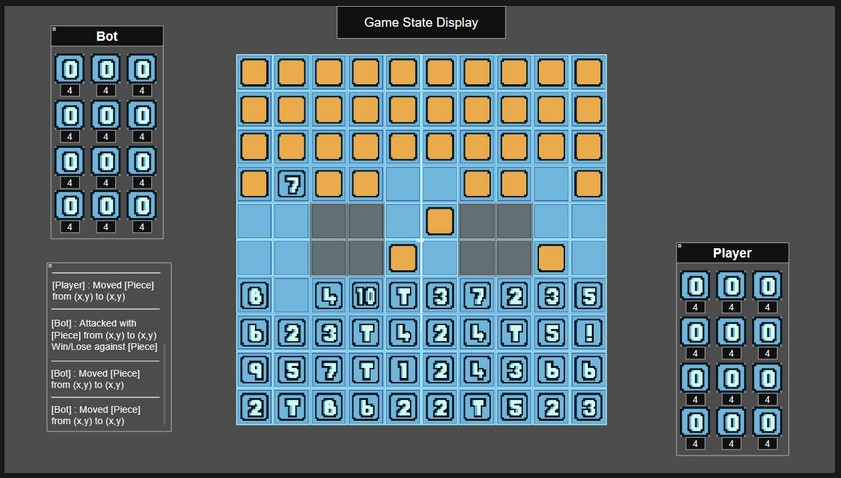
\includegraphics[width=\textwidth]{../Imagenes/boceto_partida_v1}
	\caption{Primer boceto de la interfaz de partida con indicadores laterales y texto de turno.}
	\label{fig:boceto_partida_v1}
\end{figure}

En una segunda revisión del diseño, se buscó una mayor limpieza visual. Se sustituyó el display de texto superior por un marcador de turno más iconográfico y llamativo, situando el icono del jugador actual (o el bot) en un lateral. Asimismo, los contadores de piezas se agruparon a la izquierda para liberar espacio, desplazando el historial a la derecha como aparece en la Figura \ref{fig:boceto_partida_v2}.

\begin{figure}[H]
	\centering
	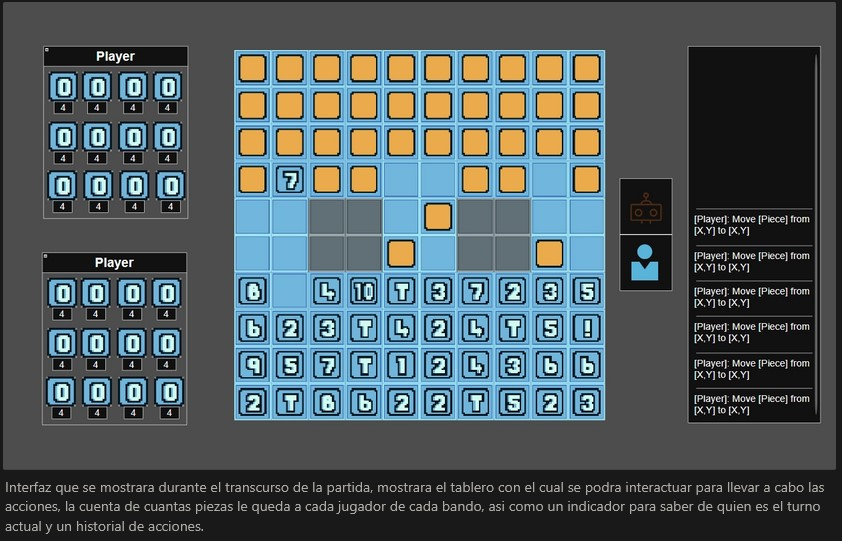
\includegraphics[width=\textwidth]{../Imagenes/boceto_partida_v2}
	\caption{Evolución del diseño de partida con indicadores visuales de turno.}
	\label{fig:boceto_partida_v2}
\end{figure}

Finalmente, la estructura definitiva eliminó el historial de movimientos. Se consideró que esta información resultaba redundante y generaba un exceso de ruido visual que no aportaba un valor crítico a la experiencia de juego, dejando como resultado final el boceto de la Figura \ref{fig:boceto_partida_v3}. En la implementación final, el marcador de turnos se simplificó de dos iconos que se iluminaban alternativamente a un único icono dinámico que cambia según el turno activo.

\begin{figure}[H]
	\centering
	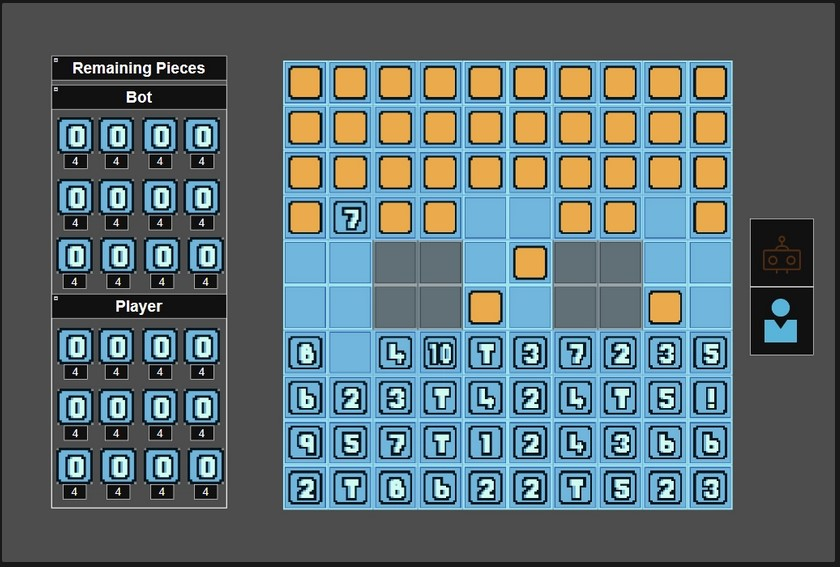
\includegraphics[width=\textwidth]{../Imagenes/boceto_partida_v3}
	\caption{Layout definitivo del boceto de la interfaz de partida.}
	\label{fig:boceto_partida_v3}
\end{figure}

% ─────────────────────────────────────────────────────────────────────────────
\subsection{Interfaz de combate y reglas}
% ─────────────────────────────────────────────────────────────────────────────

El diseño de la interfaz de combate siguió una lógica similar de simplificación. Inicialmente, se planteó como una estructura de contenedores anidados que separaban visualmente al atacante del defensor. Sin embargo, para la versión final se optó por eliminar los marcos contenedores externos, dejando los elementos de las piezas más libres y situando el mensaje del resultado del combate en la parte inferior de las mismas para no entorpecer la visión de la acción. Dicha diferencia puede apreciarse en los bocetos que aparecen en la Figura \ref{fig:boceto_comparacion_combate}.

A continuación, se presentan los bocetos que detallan el funcionamiento de los distintos estados de resolución de un combate: en la Figura \ref{fig:combate_estado1} el inicio del combate, en la Figura \ref{fig:combate_estado2} la comparación entre piezas, y en la Figura \ref{fig:combate_estado3} el resultado final antes de cerrar la interfaz.

\begin{figure}[H]
	\centering
	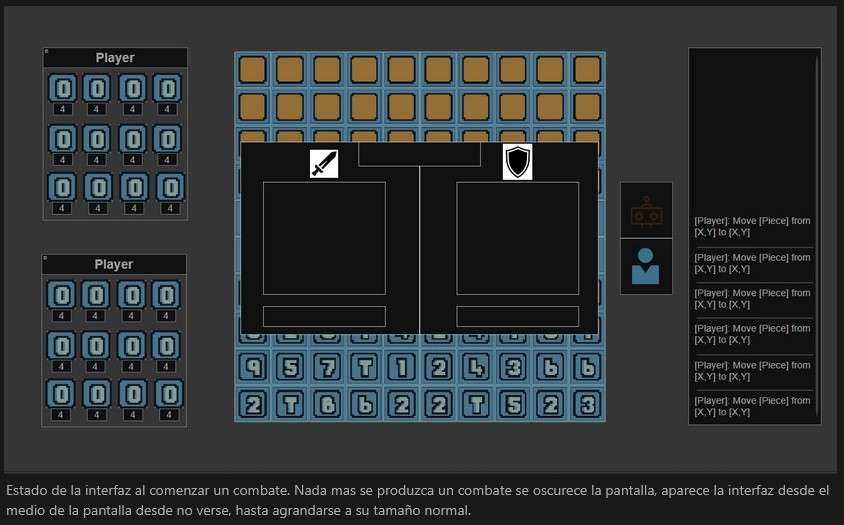
\includegraphics[width=\textwidth]{../Imagenes/combate_estado1}
	\caption{Boceto de inicio de combate: presentación de piezas.}
	\label{fig:combate_estado1}
\end{figure}

\begin{figure}[H]
	\centering
	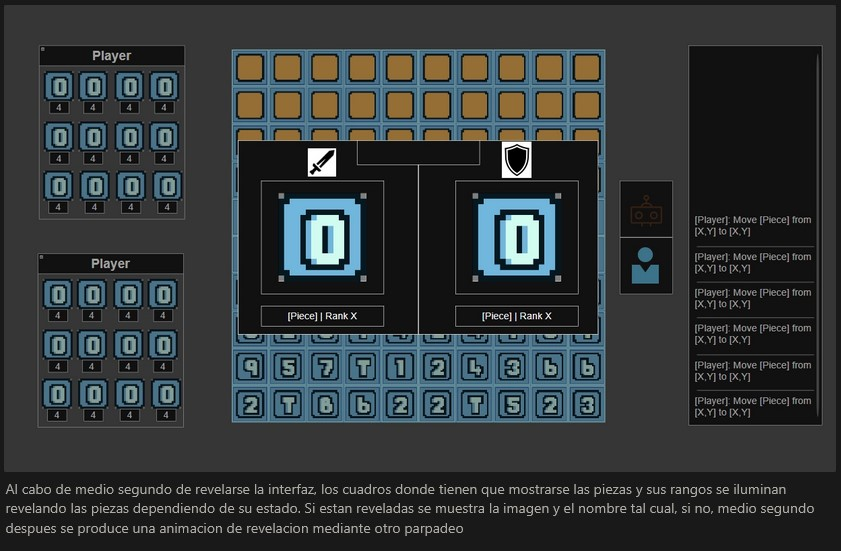
\includegraphics[width=\textwidth]{../Imagenes/combate_estado2}
	\caption{Boceto de resolución: comparación de rangos.}
	\label{fig:combate_estado2}
\end{figure}

\begin{figure}[H]
	\centering
	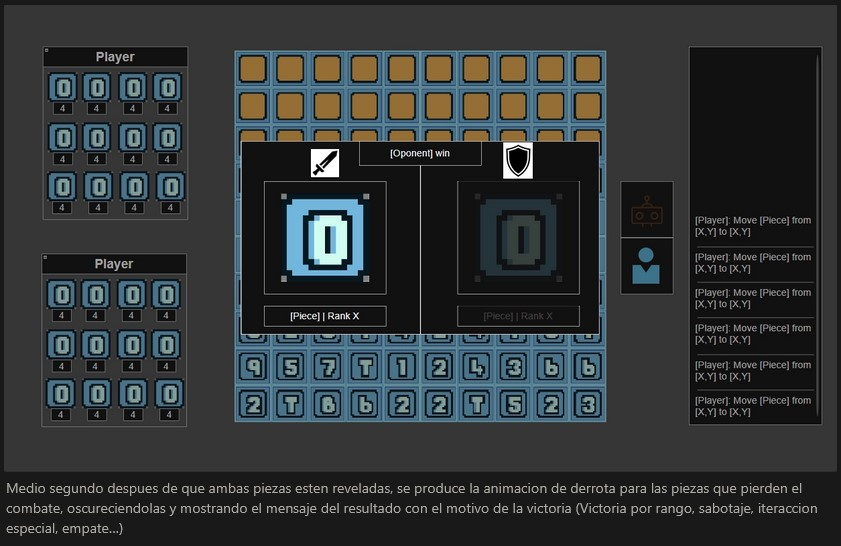
\includegraphics[width=\textwidth]{../Imagenes/combate_estado3}
	\caption{Boceto de fin de combate: pieza eliminada.}
	\label{fig:combate_estado3}
\end{figure}

\begin{figure}[H]
	\centering
	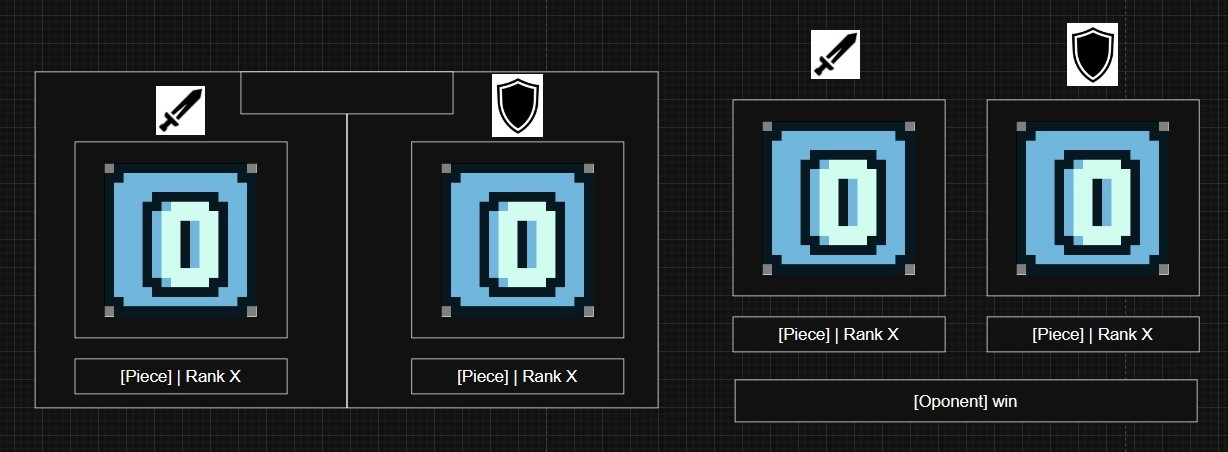
\includegraphics[width=\textwidth]{../Imagenes/boceto_comparacion_combate}
	\caption{Comparativa entre el diseño inicial de combate y el diseño final simplificado.}
	\label{fig:boceto_comparacion_combate}
\end{figure}

Por último, se diseñó el menú de pausa de la Figura \ref{fig:boceto_pausa} y la guía de reglas. Para este último, se descartó la idea inicial de un \textit{popup} único con texto denso, como el de la Figura \ref{fig:boceto_reglas}, por el de un sistema de cinco viñetas navegables. Cada viñeta aborda un aspecto específico: el objetivo principal, tipos de casillas, reglas de movimiento, reglas de combate y datos de las piezas. Este enfoque permite al jugador asimilar las mecánicas de forma progresiva.

\begin{figure}[H]
	\centering
	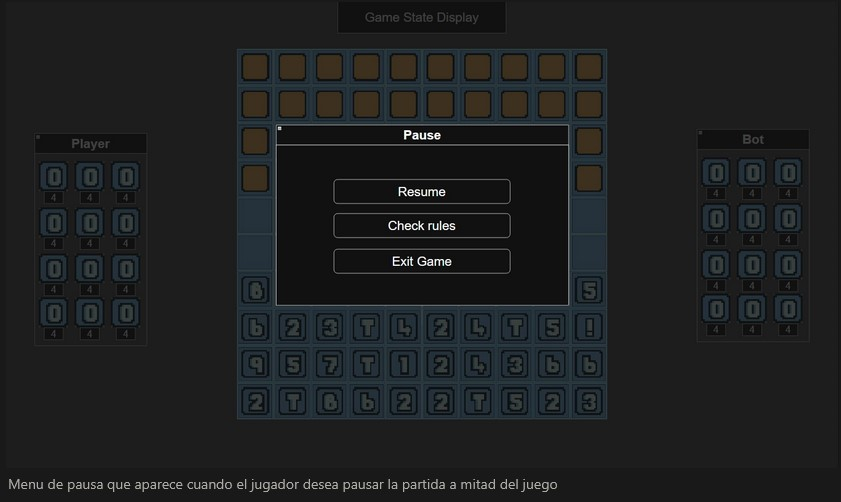
\includegraphics[width=\textwidth]{../Imagenes/boceto_pausa}
	\caption{Boceto del menú de pausa de la partida.}
	\label{fig:boceto_pausa}
\end{figure}

\begin{figure}[H]
	\centering
	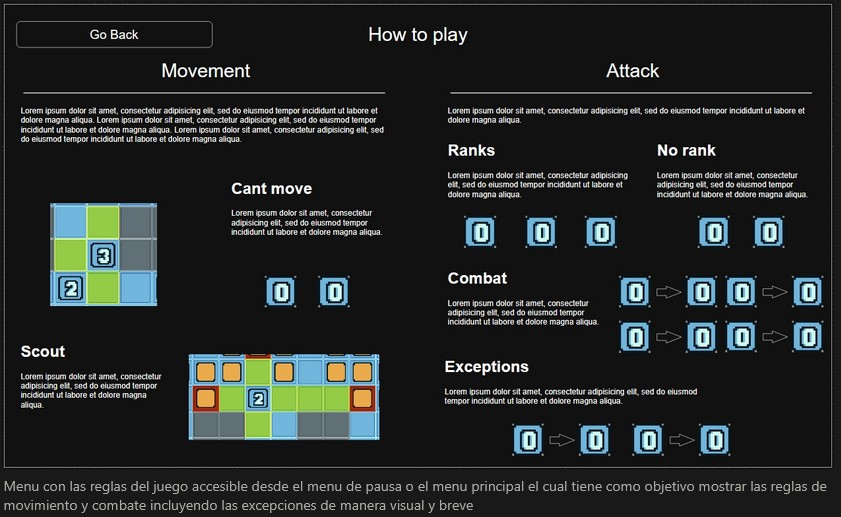
\includegraphics[width=\textwidth]{../Imagenes/boceto_reglas}
	\caption{Boceto de la interfaz de reglas con sistema de navegación por viñetas.}
	\label{fig:boceto_reglas}
\end{figure}

No se realizaron bocetos adicionales para los menús principal, de opciones o de fin de partida, dada su sencillez estructural. Cabe destacar que el diseño estético definitivo y la implementación final de todas estas interfaces que se desarrollaron a lo largo de esta iteración se detallan en el capítulo de Diseño. La iteración acabo antes del plazo establecido.

% ─────────────────────────────────────────────────────────────────────────────
\subsection{Iteración 3: Mejoras audiovisuales}
% ─────────────────────────────────────────────────────────────────────────────

Una vez consolidada la base visual y lógica, la tercera iteración se dedicó íntegramamente al apartado sonoro y al refuerzo del \textit{game feeling}. El objetivo principal fue eliminar la sensación de monotonía y vacío que presentaba el prototipo hasta el momento.

Para ello, se incorporaron pistas de música ambiental diferenciadas tanto para los menús como para el transcurso de la partida, dotando al videojuego de una atmósfera más inmersiva. En cuanto a los efectos de sonido (SFX), se implementaron tres niveles de interacción:

\begin{itemize}
	\item \textbf{Interfaz:} Sonidos sutiles de \textit{hover} y \textit{click} para que el jugador perciba qué elementos son interactuables.
	\item \textbf{Tablero:} Feedback auditivo al seleccionar y desplazar piezas, reforzando la sensación de manipulación física.
	\item \textbf{Eventos de partida:} Sonidos específicos para la revelación de piezas, derrotas en combate o cambios de estado, proporcionando una respuesta inmediata a las acciones del jugador.
\end{itemize}

Finalmente, se incluyeron fondos coherentes entre el menú principal y la escena de la partida para unificar la estética y evitar que el transcurso de la partida se sintiera visualmente vacío. A estos fondos se les aplicó un ligero efecto de \textit{parallax}, lo que aporta profundidad y una mayor sensación de pulido a la experiencia. La iteración acabo dentro antes del plazo establecido.

% ─────────────────────────────────────────────────────────────────────────────
\section{Iteración 4: Implementación del bot inteligente}
% ─────────────────────────────────────────────────────────────────────────────

La cuarta iteración se dedicó al desarrollo del sistema de inteligencia artificial, constituyendo la parte técnicamente más exigente del proyecto. El trabajo se articuló en torno a un entorno de aprendizaje por refuerzo 
implementado en Python mediante \textbf{Gymnasium} y entrenado con \textbf{MaskablePPO} de la biblioteca \textit{SB3-Contrib}.

El primer bloque de trabajo consistió en desarrollar el entorno de entrenamiento, que replica las reglas completas del videojuego de forma independiente al motor Godot. Este entorno define el espacio de observación mediante tres canales matriciales que codifican la identidad y rango de las piezas, la transitabilidad del tablero y la movilidad del agente en cada turno; así como el espacio de acciones, que cubre todos los movimientos posibles sobre el tablero. La máscara de acciones garantiza que el agente nunca seleccione un movimiento inválido durante el entrenamiento, lo que estabiliza considerablemente el proceso de aprendizaje.

El segundo bloque se centró en el entrenamiento del modelo mediante una estrategia de \textit{self-play}: el agente entrena progresivamente contra versiones anteriores de sí mismo, lo que le permite desarrollar estrategias de engaño, inferencia y gestión del riesgo de forma autónoma sin necesidad de diseñar manualmente una función de evaluación del tablero. Cada versión del modelo se guarda con una marca temporal y el entrenamiento puede reanudarse desde el último punto de control.

El tercer bloque consistió en la integración del modelo entrenado con el motor Godot. Se implementó un \texttt{BotController} en C\# que lanza un subproceso Python en segundo plano al iniciar la partida, carga el archivo \texttt{.zip} del modelo y se comunica con él mediante un canal de entrada y salida estándar para solicitar la acción del bot en cada turno. Esta arquitectura mantiene el entorno de inferencia completamente desacoplado del motor, de modo que actualizar el modelo no requiere modificar el código del videojuego. La iteración finalizó un día antes del plazo previsto.

% ─────────────────────────────────────────────────────────────────────────────
\section{Iteración 5: Pulido final}
% ─────────────────────────────────────────────────────────────────────────────

La quinta y última iteración se dedicó a la consolidación del sistema completo, abordando los aspectos de calidad y estabilidad que habían quedado pendientes en fases anteriores.

En el apartado de rendimiento, se revisaron los ciclos de actualización de los nodos más activos durante la partida y se optimizó la gestión de señales y eventos para reducir el número de llamadas innecesarias en cada fotograma. El resultado fue una ejecución fluida y estable en el hardware mínimo especificado en los requisitos no funcionales.

La revisión del feedback al jugador permitió detectar y corregir varios casos en los que la respuesta visual o sonora a una acción no era suficientemente clara, especialmente en situaciones de combate entre piezas reveladas previamente y en la transición entre el turno del jugador y el del bot. Se ajustaron los tiempos de animación y se reforzaron los efectos sonoros asociados a estos momentos para mejorar la legibilidad de la partida.

En cuanto a la corrección de errores, se resolvieron varios casos límite relacionados con la regla antioscilación en situaciones de tablero muy congestionado, y se corrigió un comportamiento incorrecto del explorador al intentar moverse a través de casillas ocupadas en determinadas configuraciones. Las pruebas de integración finales verificaron el comportamiento completo del sistema de principio a fin, desde el despliegue inicial hasta todas las condiciones de victoria posibles, sin detectar errores adicionales. La iteración se completó en la fecha prevista, cerrando el desarrollo del proyecto dentro del plazo establecido.